\chapter{系统拓扑结构研究}
\label{cha:SystemTopology}

经过\autoref{cha:Introduction}的分析,本文确立了研究目标和研究内容,其中梯级系统拓扑结构的选择是直接关系到梯级系统能否安全高效运行的先决条件。一个具有不合理拓扑结构的梯级系统甚至不能正常运行。本章以现有成熟光热发电技术为基础,经过对太阳能梯级集热发电的多种考虑因素的分析和排除,选择应用于梯级系统的各种技术方案及相关部件,经过合理的布局,确定有效的太阳能梯级集热发电的拓扑结构方案。

现有的经过商业验证的太阳能热发电技术有三种——太阳能槽式发电,太阳能碟式发电和太阳能塔式发电。
由于太阳能塔式发电系统占地面积较大,投资成本太高,考虑到未来需要搭建太阳能梯级集热发电示范系统,本文仅选择两种太阳能光热发电技术(太阳能槽式发电和太阳能碟式发电)作为太阳能梯级集热发电系统设计的基本系统。为了实现对太阳能碟式集热器获得的高温热量进行梯级利用,采用空气(或氮气)作为太阳能碟式发电系统的传热介质来传输所收集的热量。
\begin{figure}[htbp]
\centering
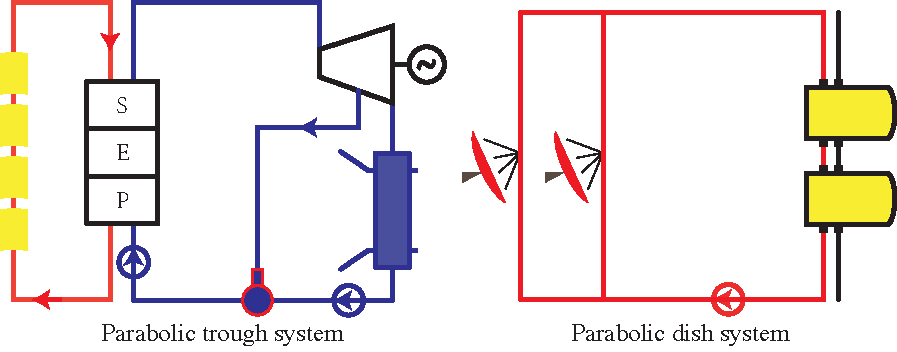
\includegraphics[width=0.8\textwidth]{fig/PTPD.pdf}
\caption{太阳能槽式发电系统和太阳能碟式发电系统结构示意图}
\label{fig:PTPD}
\end{figure}
典型的太阳能槽式发电系统和太阳能碟式发电系统的结构示意图如\autoref{fig:PTPD}所示。为使本文中的系统结构图更加清晰一致,\autoref{fig:Legends}列出了太阳能光热发电系统中可能出现的所有元件的图例。

\begin{figure}[t!]
\centering
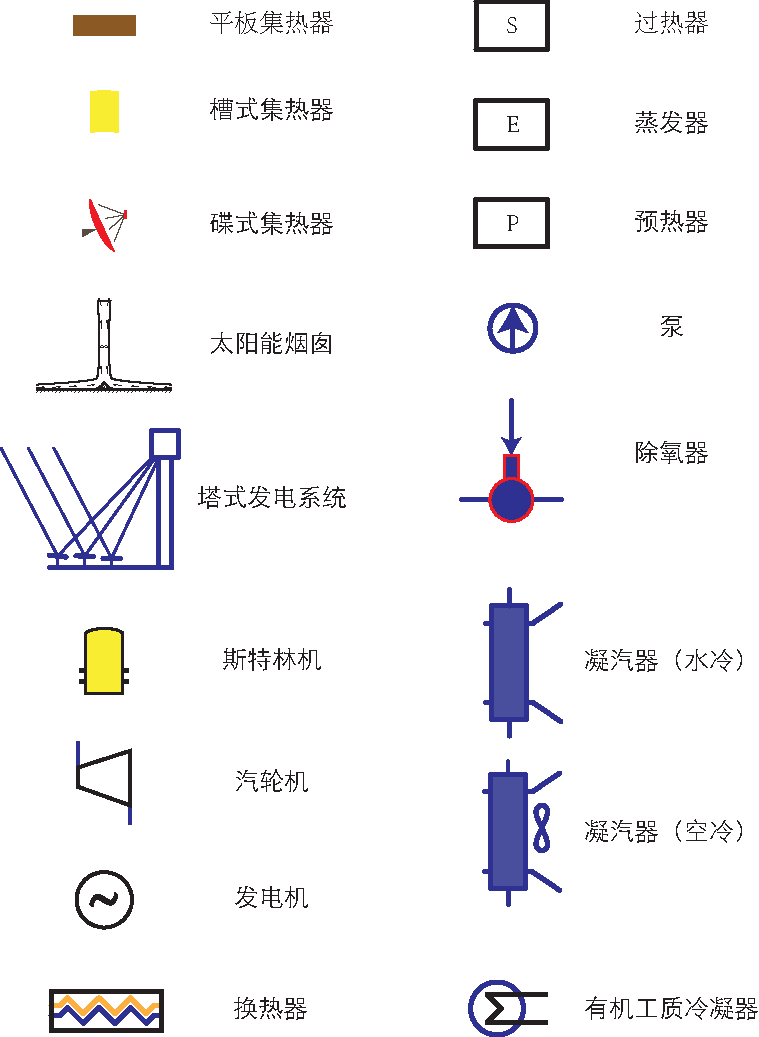
\includegraphics[width=0.8\textwidth]{fig/Legends.pdf}
\caption{太阳能光热发电系统中的元件列表}
\label{fig:Legends}
\end{figure}

利用这两种基本系统,通过选择不同的系统拓扑结构,来实现能量的梯级收集和梯级利用。由于梯级系统的拓扑结构需要考虑多种方案,例如朗肯循环结构的选择、与太阳能烟囱技术的集成、多种集热方式的集成、朗肯循环与斯特林循环的集成等,梯级系统可以组合的拓扑结构的数量非常之多。为了获得最合适的梯级系统拓扑结构,需要从可行性、经济性等角度仔细逐个分析这些因素。需要说明的是,本文进行的研究没有考虑采用蓄热系统,这是因为:(1) 本文重点在于从理论上分析梯级系统能量的梯级收集和梯级利用,分析的条件是基于系统稳态运行的假设,所以无需设置蓄热器。(2) 蓄热器的存在将会改变系统的集热温度和供热温度的匹配性,给系统的分析带来额外的工作量。(3) 本文拟建立的梯级示范系统仅用于实验研究,暂不考虑将发出的电能并网,而蓄热系统的加入会产生额外的成本。(4) 蓄热系统可以在后续研究工作中引入,而不影响本文的研究内容和结论。

\section{基于朗肯循环的系统结构}
\label{sec:RankineCycleBased}

朗肯循环的系统结构主要受朗肯循环工质的影响,水工质朗肯循环(SRC)太阳能光热系统的典型结构示意图和有机工质朗肯循环(ORC)太阳能光热系统的典型结构示意图分别如\autoref{fig:TypicalSteamRankineSolarSystem}和\autoref{fig:TypicalOrganicRankineSolarSystem}
所示。本节主要研究朗肯循环工质的选择问题。

\begin{figure}[htbp]
\centering
	\begin{subfigure}[b]{0.4\columnwidth}
	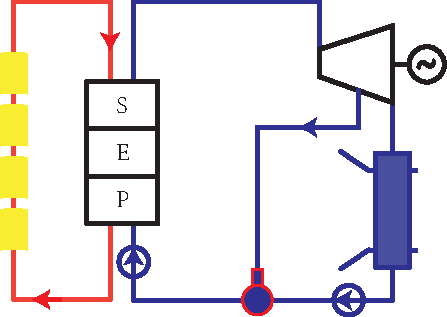
\includegraphics[width = \columnwidth]{fig/TypicalSteamRankineSolarSystem}
	\caption{}\label{fig:TypicalSteamRankineSolarSystem}
	\end{subfigure}
	~
\begin{subfigure}[b]{0.4\columnwidth}
	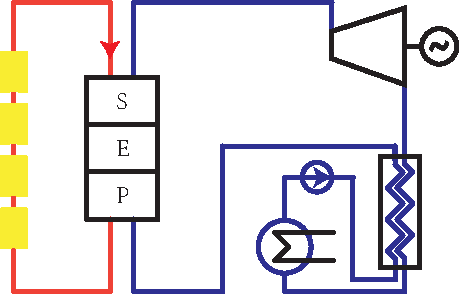
\includegraphics[width = \columnwidth]{fig/TypicalOrganicRankineSolarSystem}
	\caption{}\label{fig:TypicalOrganicRankineSolarSystem}
	\end{subfigure}
	\caption{采用SRC和ORC的太阳能光热系统的典型结构示意图}
	\label{fig:TwoTypesOfRankineCycle}
\end{figure}


\subsection{理想朗肯循环工质特点}
\label{sec:IdealRankineCycleFluid}

\begin{figure}[!ht]
\centering 
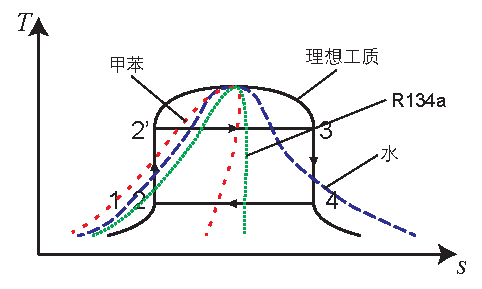
\includegraphics[width=0.5\textwidth]{fig/idealTs}
\caption{用于朗肯循环的理想工质的温熵图}
\label{fig:idealTs}
\end{figure}

应用于朗肯循环的不同工质的温熵曲线如\autoref{fig:idealTs}所示。需要说明的是,图中各曲线只是用于表示不同工质的饱和曲线形状,曲线对应的熵值和温度不代表其真实熵值和温度,也不能用于不同工质之间的比较。其中,理想工质具有以下特点\cite{Abbin1977}:
\begin{itemize}

	\item 饱和液体的比热容要小,这样\autoref{fig:idealTs}中的曲线2-2'才接近竖直。
	\item 临界点温度要高于最高运行温度,以使所有的吸热过程都发生在临界点温度以下。
	\item 最高运行温度所对应的饱和蒸汽压力应该适中,以便安全运行并有利于降低设备的制造成本。
	\item 凝气温度下对应的蒸气压力应该高于大气压,以避免空气泄漏到系统中。
	\item 状态点4的蒸气的密度应该较大,这样可以避免大尺寸的汽轮机叶片,壳体和换热器。
	\item \autoref{fig:idealTs}中气态饱和曲线3-4应该接近竖直,从而避免汽轮机中的工质膨胀进入湿蒸汽区($ds/dT < 0$的情况)或是过热区($ds/dT > 0$的情况)。
	\item 对于小功率汽轮机的应用,工质应该具有较高的分子量以便于减小汽轮机的转速和(或)减少级的数量,并且允许合适的质量流量和汽轮机喷嘴面积。
	\item 工质在常温常压下为液体,以便于运输和控制。
	\item 工质的凝固点应该低于工作的环境温度。
	\item 工质具有良好的传热性能,价格便宜,在最高操作温度下热稳定较好,不易燃烧,无腐蚀性,无毒性等。
\end{itemize}

\subsection{水工质朗肯循环和有机工质朗肯循环的特点}
\label{sec:RankineCycleFluid}

水是朗肯循环中最常用的工质,水工质朗肯循环的各部件相关的技术比其他工质更为成熟。水的价格便宜(虽然锅炉级的水必须是高度蒸馏的,因此成本比自来水高),水工质朗肯循环的高压部分的密封并没有其它工质那么重要。此外,蒸汽的不易燃性和可用性是其额外的优点。因为它的临界温度和压力分别为374$\mathrm{^\circ C}$和22$\,\mathrm{MPa}$,它可以在中等压力下实现较高温度的等温吸热。

水工质朗肯循环也存在一些缺点。蒸汽的低温特性并不理想,因为蒸汽在常温下具有很低的蒸气压和密度(参见\autoref{tab:waterT_P_D})。对于低压部件,保持密封性,防止空气泄漏是设计中需要注意的问题。
\begin{table}[htbp]
\setlength{\abovecaptionskip}{0pt}
	\caption{不同温度下饱和蒸汽的压力和密度}
	\centering
	\begin{tabular}{cccccccccc}
		\toprule	
		    $T$(K)    &	373.15	    &    363.15    &    353.15    &    343.15    &    333.15    &    323.15    &    313.15    &    303.15    &    293.15\\
		\midrule	
		    $p$(Pa)    &    101322        &    70117    &    47373    &    31176    &    19932    &    12344    &    7381    &    4246    &    2339\\
		    $\rho$($\mathrm{kg/m^3}$)    &    0.5982        &    0.4239    &    0.2937    &    0.1984    &    0.1304    &    0.0831    &    0.0512    &    0.0304    &    0.0173\\
		\bottomrule
	\end{tabular}
	\label{tab:waterT_P_D}
\end{table}

有机工质朗肯循环也可应用于太阳能槽式发电,取代常见的水工质朗肯循环。ORC可以在小功率和低集热温度的条件下进行发电,因此可以用于生产低成本,小规模的分布式CSP装置。ORC中使用的大多数有机工质是干流体(温熵图上$ds/dT > 0$)。汽轮机出口的气体具有一定的过热度,由于汽轮机出口温度高于冷凝器温度,所以可以将一部分热量传递给压缩过的液态有机工质。\autoref{fig:TypicalOrganicRankineSolarSystem}中的回热器就是为了回收利用这一部分热量而设计的,回热器为过热蒸气-过冷液体换热器。
%典型的有机工质太阳能光热系统结构示意图如\autoref{fig:TypicalOrganicRankineSolarSystem}所示。

%Compared with steam for the Rankine cycle, it has the following advantages:
与水工质朗肯循环相比,它具有以下优点:
\begin{itemize}
%  \item  Small turbine head allows for moderate shaft speed and a single- or two-stage design.
    \item 有机工质具有更低的沸点,在常温下具有更高的饱和蒸汽压力,它更适宜于回收低温废热。此外,其密度和比热容较小,所需要的汽轮机、管道和换热面积都较小,这些都有利于降低制造成本。
    \item 有机工质在膨胀的过程中温降很小,这有利于减少热应力导致的各种问题。
    \item 有机工质具有很低的凝固点,这意味着即使在寒冷地区也不需要针对有机工质做防冻措施。
    \item 汽轮机的排气没有湿度(干气体)。所以无需过热,饱和蒸气就可以用作汽轮机的主气。有机工质汽轮机不会发生由于湿蒸气存在液滴给高速旋转的叶片带来的腐蚀现象。
    \item 相同温度下,有机工质的凝汽压力比水工质高。常温下,有机工质可以在高于大气压的条件下凝结。系统压力可以保持在大气压以上运行,这就可以避免空气泄漏进入系统。这也意味着有机工质朗肯循环不再需要除氧器。
    \item 较低的系统运行压力便于汽轮机实现一体化设计。
    \item 有机工质流体具有比蒸汽更低的声速,汽轮机可以在较低转速下达到较好的气动力学性能。在中等转速和单级或双级的设计条件下可以实现小型汽轮机应用。
  \end{itemize}
  
\subsection{朗肯循环工质的选择}
\begin{figure}[!ht]
\centering 
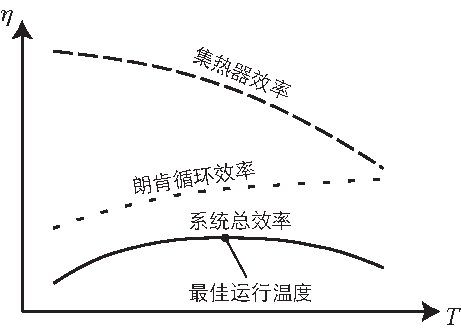
\includegraphics[width=0.5\textwidth]{fig/Efficiency}
\caption{不同运行温度下的效率曲线}\label{fig:Efficiency}
\end{figure}
选择太阳能光热系统朗肯循环的工作流体时需要考虑两个重要方面:
\begin{enumerate}
  \item 选择的工作流体易于在最佳运行温度条件下运行。
 对于朗肯循环太阳能光热系统,集热器效率随着工作温度的升高而降低,朗肯循环的效率随着工作温度的升高而升高,系统的总效率存在如\autoref{fig:Efficiency}所示的最佳工作温度。工作流体应当有利于达到该最佳工作温度。    
  \item 如果使用传热流体,则传热流体的状态需要和热力循环的工作流体的状态相匹配。
  一方面,工作流体的工作温度应该低于传热流体的集热温度。另一方面,工作流体的工作温度不应该比传热流体的集热温度低很多,以避免换热过程中产生大量的㶲损失。
\end{enumerate}

\autoref{sec:RankineCycleFluid}中详细介绍了水和有机工质作为朗肯循环的工作流体所带来的优缺点。对于低参数和小容量的配电发电,有机工质将是更好的选择,否则水是更好的选择。Bao和Zhao\cite{Bao2013}对工作流体的选择(包括纯液体和混合液)进行了全面的综述。在该综述中,考虑了许多因素,如操作条件,工作流体的特性,设备结构和环境安全等。
必须强调的是,工作流体的种类(主要是干流体或湿流体)会影响系统的运行和布局。

\section{槽式朗肯循环与太阳能烟囱技术集成的系统结构}
\label{sec:sc}

太阳能烟囱电站也被称为太阳能热气流电站,它直接(不聚光)利用太阳产生的热能来发电。太阳能烟囱发电系统由太阳能集热棚、太阳能烟囱和涡轮机发电机组3个基本部分构成,典型的太阳能烟囱电站的示意图如\autoref{fig:SolarChimney}所示。太阳能烟囱电站建立在太阳辐射强度高,土地保温性能好的地区。集热棚离地面有一定距离,其外围周边是开放的。太阳能烟囱和集热棚连接,位于集热棚中央。涡轮机发电机组位于烟囱底部。
在这种电站中,空气在半透明的集热棚下因温室效应而升温。集热棚的周边是开放的,外部空气由于密度分布不同而流入集热棚,然后在浮力的作用下热空气流入烟囱产生热气流。在气流的路径上设置有涡轮机发电机组,用于将气流的动能转化为电能。

\begin{figure}[!ht]
\centering 
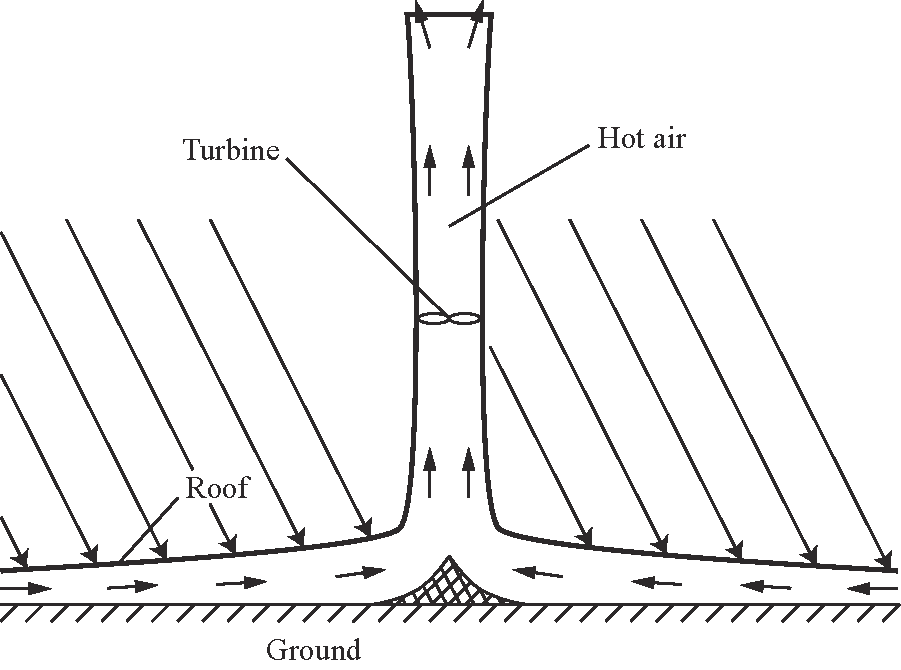
\includegraphics[width=0.5\textwidth]{fig/SolarChimney}
\caption{太阳能烟囱电站的结构示意图}\label{fig:SolarChimney}
\end{figure}

太阳能烟囱可以利用低温热源(低品位能源)发电。因此,槽式系统和太阳能烟囱的组合可以作为能源梯级利用的有效途径。在组合系统中,朗肯循环中的冷凝器采用空冷。空冷风扇将冷却过冷凝器的热空气从太阳能烟囱的周边吹入太阳能烟囱发电厂。热气流汇聚在烟囱底部,在浮力作用下向上流动,带动烟囱内的涡轮机发电机组,从而实现朗肯循环凝结热的有效利用。
\autoref{fig:CombinedSolarChimney}显示了一个槽式系统和太阳能烟囱技术集成的例子。

\begin{figure}[!ht]
\centering 
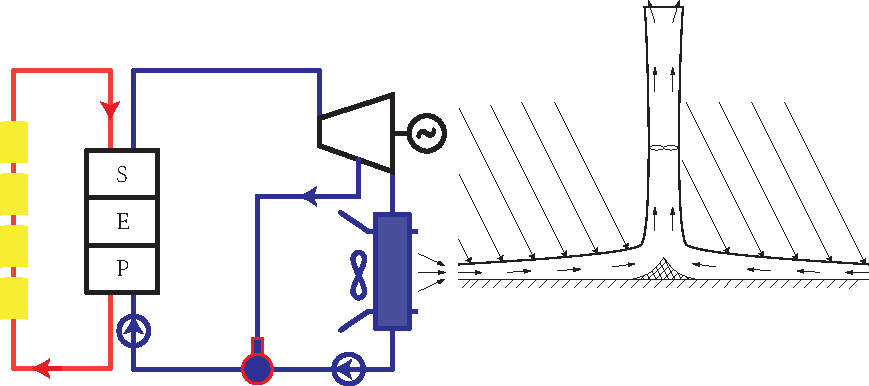
\includegraphics[width=0.7\textwidth]{fig/CombinedSolarChimney}
\caption{槽式系统和太阳能烟囱组合结构示意图}\label{fig:CombinedSolarChimney}
\end{figure}
然而,目前的太阳能烟囱系统的效率非常低。Bilgen和Rheault利用MATLAB建立了5$\,\mathrm{MW}$的太阳能烟囱电站模型,并同Schlaich的模型进行了比较\cite{Bilgen2005}。他们对不同地理位置,不同烟囱高度的太阳能烟囱电站进行了模拟分析。其主要设计数据及计算结果如\autoref{tab:sc}所示。 初步的设计参数为太阳辐射强度为1000$\,\mathrm{W/m^2}$,额定功率为5$\,\mathrm{MW}$。从表中可以发现,烟囱效率和系统总效率都很低,太阳能烟囱技术仍处于初步发展阶段。
\begin{table}[htbp]
\setlength{\abovecaptionskip}{0pt}
	\caption{太阳能烟囱设计参数及模拟结果}
	\centering
	\begin{tabular}{ccccc}
		\toprule
			&渥太华    &温尼伯    &埃德蒙顿    &Schlaich的模型\\
		\midrule
		集热棚直径 (m)    &	--	&	--	&	--	&	1110 \\
  集热棚面积 ($\mathrm{m^2}$)    & 950000    & 950000	&	950000	&	950000\\
  烟囱高度 (m)    &123    &60    &    35&    547\\
%  集热棚高度 (m)    &848    &975    &1024    &    -\\
  烟囱直径 (m)    &54    &54    &54    &54\\
  集热棚内温升 ($\mathrm{^\circ C}$)    &25.9    &25.9    &25.9    &25.9\\
  气流速度 (m/s)&9.1    &9.1    &9.1    &9.1\\
  总压头 (Pa)&518.3    &518.3    &518.3    &383.3\\
  平均效率\\
  集热棚 (\%)    &56.00    &56.00    &56.00    &56.24\\
  烟囱 (\%)    &1.82    &1.82    &1.82    &1.45\\
  涡轮机 (\%)    &77.0    &77.0    &77.0    &77.0\\
  系统整体 (\%)    &0.79    &0.79    &0.79    &0.63\\
		\bottomrule
	\end{tabular}
	\label{tab:sc}
\end{table}
 
另外,太阳能烟囱成本高,占地面积大,不利于今后搭建太阳能梯级集热发电示范系统。鉴于这些,梯级系统不采用太阳能烟囱技术。

\section{多种集热方式集成的系统结构}
\label{sec:csc}
考虑到每种类型的集热器都有其适宜的工作温度范围,集成使用多种集热方式,采用多种集热器逐步加热传热流体是实现梯级集热的可行方案。
槽式集热器和菲涅耳集热器更适合于低温集热,碟式集热器和塔式集热器更适合于高温集热。串联连接不同类型的集热器可以有效利用它们各自的优点。\autoref{fig:SeriesCollector}给出了一个采用集热器串联连接的梯级系统的方案。在这个系统中,空气作为传热介质在流入碟式集热器之前先被槽式集热器预热。槽式集热器用于收集低温热能,碟式集热器用于收集高温热能。

在这种方案中,空气依次在槽式集热器和碟式集热器中被加热。为斯特林机提供热量后,热空气流入换热器为朗肯循环提供热量。在这种拓扑结构中,空气被用作太阳能槽的传热流体,这个想法目前只有少数研究人员进行了数值和实验研究,至今还没有商业应用\cite{Good2015,Good2016}。这种技术最大的技术难题在于,空气导热系数低,热容量低,导致系统效率非常低。由于该拓扑结构使用了尚不成熟的空气槽式集热技术,故不采用这种方案。
\begin{figure}[ht!]
\centering 
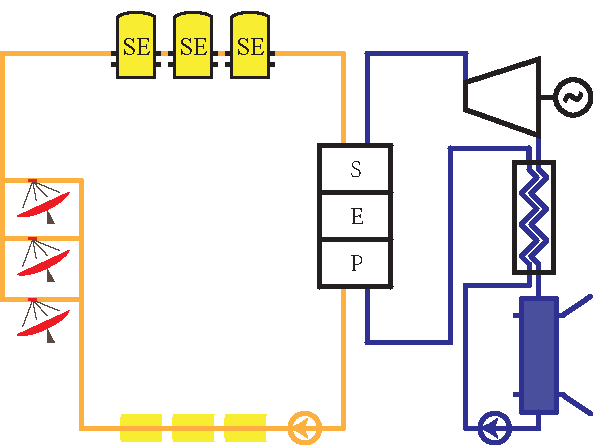
\includegraphics[width=0.6\textwidth]{fig/SeriesCollector}
\caption{一种采用集热器串联连接的梯级系统方案}\label{fig:SeriesCollector}
\end{figure}

有的太阳能塔式电厂采用水作为传热流体(如Solar One电厂),这时可以利用平板式太阳能集热器和(或)槽式集热器作为低温段的集热器。系统结构图如\autoref{fig:seriesCollection}所示,冷凝水由平板式集热器加热,给水由槽式集热器加热。与太阳能塔式电厂相比,平板式集热器和槽式集热器收集低温热量的单位热成本要低很多。平板式集热器和槽式集热器的串联连接加入可以有效降低系统发电成本。虽然该方案有很好的前景,值得进一步研究,但本文的梯级系统不考虑采用太阳能塔式系统,所以该方案留给后续研究工作。
\begin{figure}[htbp]
\centering 
\includegraphics[width=0.6\textwidth]{fig/SeriesCollection}
\caption{采用多种型式集热器串联连接的太阳能塔式发电系统}\label{fig:seriesCollection}
\end{figure}

\section{朗肯循环与斯特林循环集成的系统结构}

\subsection{回路间传热的系统结构}
\label{sec:hebc}

对于\autoref{fig:PTPD}中的太阳能碟式发电系统,热空气为斯特林机提供热量后还有很高的温度,可以通过设置换热器在回路间传热,实现能量的梯级利用。根据换热回路的不同,可以在太阳能梯级系统中设置两种类型的换热器。

第一种是在空气回路和导热油回路之间使用的空气-导热油换热器。\autoref{fig:air-oil}是使用了这种换热器的一个梯级系统方案。在这个系统中,热空气在为斯特林机组供热后,再流过空气-导热油换热器为导热油提供热量。

在这种方案中,空气为导热油提供热量。从几个方面来看,这是不经济的。首先,此方案并不能进一步提高导热油的温度。导热油的极限温度受到本身物质属性的限制,而并非受限于槽式集热器,槽式集热器的集热温度可以超过这个值。在高温条件下,油品可能会变质,蒸发,分解,对系统的安全稳定运行产生不利影响。其次,使用碟式集热器为导热油提供热量是不经济的,因为碟式集热器是为了收集更高温度的热量而设计的,与槽式集热器相比,它在收集中低温热量时效益更低。

\begin{figure}[ht]
\centering 
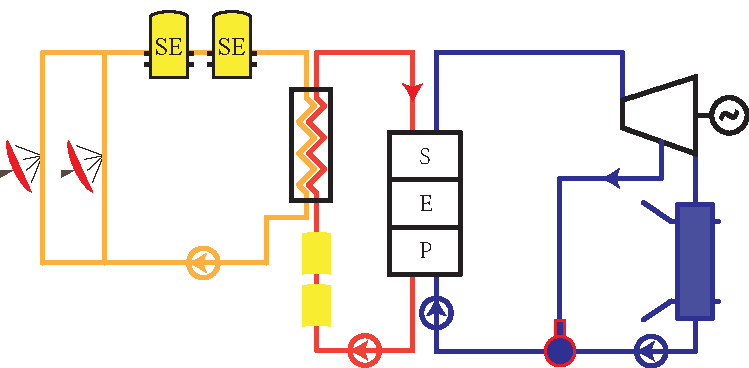
\includegraphics[width=0.7\textwidth]{fig/air-oil}
\caption{使用空气-导热油换热器的太阳能光热系统示意图}\label{fig:air-oil}
\end{figure}

\begin{figure}[htbp]
\centering
	\begin{subfigure}[b]{0.4\columnwidth}
	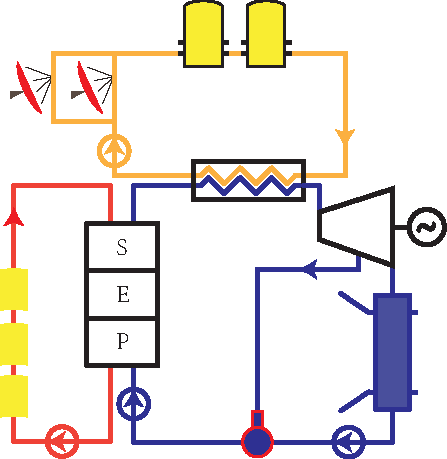
\includegraphics[width = \columnwidth]{fig/air-water1}
	\caption{}\label{fig:air-water_1}
	\end{subfigure}
	~
\begin{subfigure}[b]{0.4\columnwidth}
	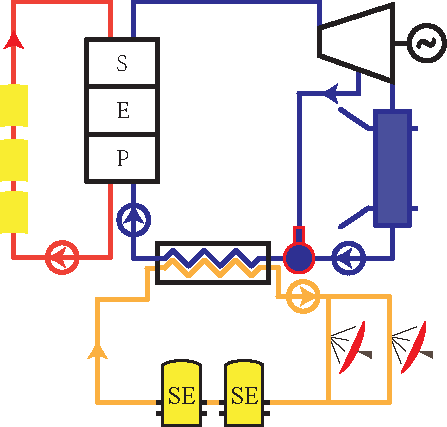
\includegraphics[width = \columnwidth]{fig/air-water2}
	\caption{}
	\label{fig:air-water_2}
	\end{subfigure}
	\caption{两种使用了空气-水换热器的梯级系统案例}
	\label{fig:air-water}
\end{figure}

第二种是在空气回路和水回路之间使用的空气-水换热器。\autoref{fig:air-water_1}和\autoref{fig:air-water_2}是使用了这种换热器的两个梯级系统方案。\autoref{fig:air-water_1}中,热空气在为斯特林机组供热后,再流经空气-水换热器,为水的过热过程提供热量。\autoref{fig:air-water_2}中,热空气在为斯特林机组供热后,再流经空气-水换热器,为水的预热过程提供热量。

在这种方案中,空气为水提供热量。\autoref{fig:air-water}给出了两种使用空气-水换热器的太阳能梯级系统方案。其中,\autoref{fig:air-water_1}给出的是使用加热过斯特林机之后的热空气来继续为过热蒸汽提供热量的方案。这是可行的,因为热空气可以提升水的吸热过程的平均温度从而提高朗肯循环的效率。另一方面,在传统的太阳能槽式系统中,主蒸汽温度受到导热油极限温度的限制,这不利于提升朗肯循环的效率。在这个梯级系统中,朗肯循环的主蒸汽温度可以提高到高于400$\mathrm{^\circ C}$以消除导热油极限温度带来的负面影响。
这一系统方案将作为主要研究方案在接下来的内容里详细讨论。\autoref{fig:air-water_2}给出的是使用加热过斯特林机后的热空气预热给水的方案。由于斯特林机出口的空气温度较高,而朗肯循环的给水温度较低,二者之间存在很大的温差。如果采用此方案,则换热过程产生的㶲损很大。此外,由于给水温度的提升导致太阳能场内的导热油的平均温度也会有所上升,这将降低太阳能场的集热效率,进而降低整个梯级系统的效率。

\subsection{循环之间热量利用的系统结构}
\label{sec:HRBC}

根据热力学第二定律,不可能从单一热源吸热使之完全转换为有用的功而不产生其他影响。对于热机,它同时需要热源和冷源来将热能转化为机械能。典型热机的热功转换图如\autoref{fig:engines}所示。在热力循环中,从热源吸收的热量,只有一部分可以通过热机转化为机械功,其它部分需要传递到冷源。卡诺定理从根本上限制了与热源温度和冷源温度有关的热功转换比,即$\dfrac{W}{Q_H} \leqslant \dfrac{T_H - T_C}{T_H}$,其中$T_H$和$T_C$的单位为$\mathrm{K}$。
\begin{figure}[htb]
\centering 
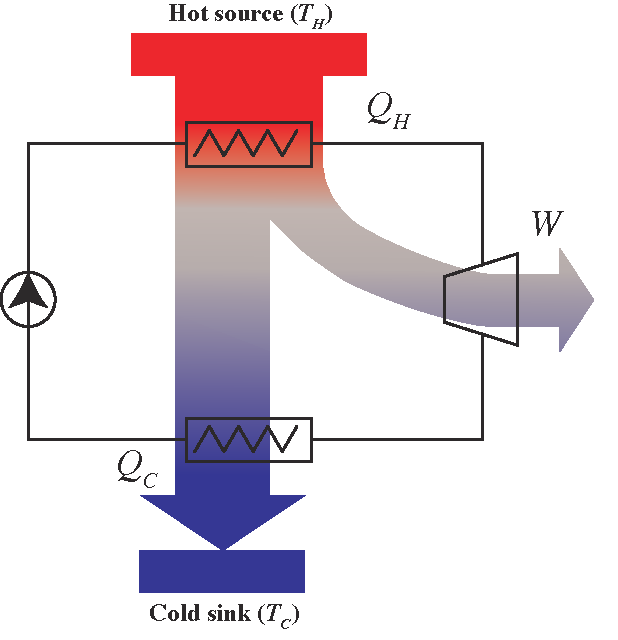
\includegraphics[width=0.5\textwidth]{fig/engines}
\caption{典型热机的热功转换图}
\label{fig:engines}
\end{figure}

不同的热机采用不同的热力循环来实现热功转换,它们有着不同的最佳工作温度。朗肯循环的最佳工作温度较低,斯特林循环的最佳工作温度较高。太阳能光热应用中斯特林循环和朗肯循环的$T$-$s$图如\autoref{fig:cycles}所示。
\begin{figure}[htb]
\centering 
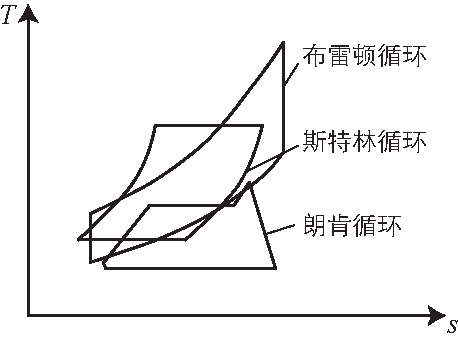
\includegraphics[width=0.5\textwidth]{fig/cycles}
\caption{太阳能光热应用中斯特林循环和朗肯循环热力循环的$T$-$s$图}\label{fig:cycles}
\end{figure}

由于每个热力循环都具有吸热和放热过程,因此可以组合多种热力循环,使一个循环(底部循环)吸收利用另一个循环(顶部循环)释放的热量,不同的循环可以耦合起来用于梯级发电。
\begin{figure}[htbp]
\centering
	\begin{subfigure}[b]{0.4\columnwidth}
	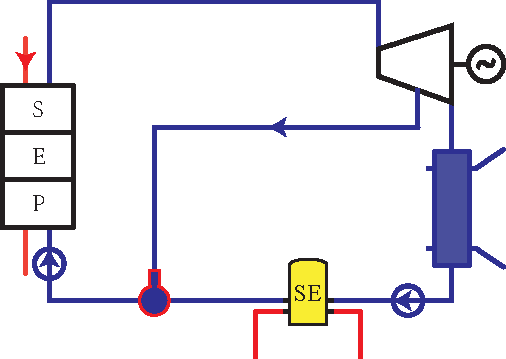
\includegraphics[width = \columnwidth]{fig/Stirling-Rankine}
	\caption{}\label{fig:Stirling-Rankine}
	\end{subfigure}
	~
\begin{subfigure}[b]{0.4\columnwidth}
	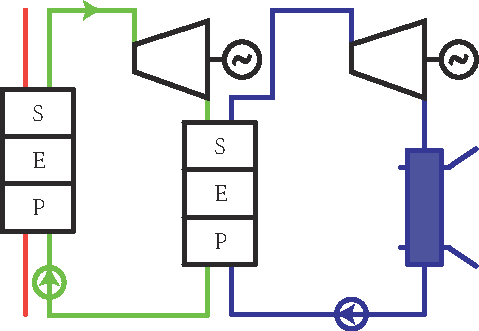
\includegraphics[width = \columnwidth]{fig/SeriesRankine}
	\caption{}\label{fig:Rankine-Rankine}
	\end{subfigure}
	\caption{采用多个热力循环之间热量回收利用的梯级系统结构图}
	\label{fig:coupledCycles}
\end{figure}

\autoref{fig:coupledCycles}给出了热力循环之间热量回收利用的梯级系统的两种系统结构。
传统的斯特林机为了提高性能,使用冷却水来吸收斯特林机释放的热量,吸收的热量往往被浪费掉而没有回收利用。
在\autoref{fig:Stirling-Rankine}中,采用朗肯循环的凝结液来冷却斯特林机。斯特林循环排出的热量可以通过朗肯循环回收利用。
对于有机朗肯循环,不同的工作流体决定循环的工作温度区间。用一个有机朗肯循环重复利用另一个有机朗肯循环的凝结热是可行的。在\autoref{fig:Rankine-Rankine}中,两个有机朗肯循环耦合在一起用于发电。底部循环利用顶部循环的凝结热来实现预热,蒸发和过热,再利用朗肯循环发电。

\section{选定的梯级系统拓扑结构}
\label{sec:sst}

考虑了以上各节中的技术方案,本文选择了两个系统拓扑结构进行太阳能梯级集热发电技术的研究,其系统结构图如\autoref{fig:CascadeSystems}所示。

%第二种方案需要考虑是否用两个空气换热器
\begin{figure}[htbp]
\centering
	\begin{subfigure}[b]{0.4\columnwidth}
	\includegraphics[width = \columnwidth]{fig/CascadeSystem1}
	\caption{}\label{fig:CascadeSystem1}
	\end{subfigure}
	~
\begin{subfigure}[b]{0.4\columnwidth}
	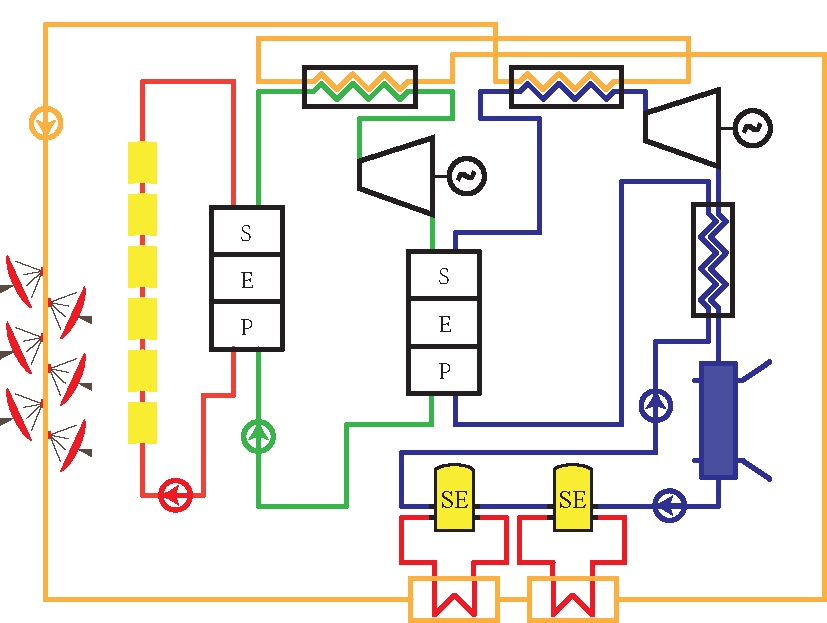
\includegraphics[width = \columnwidth]{fig/CascadeSystem2}
	\caption{}\label{fig:CascadeSystem2}
	\end{subfigure}
	\caption{两种选定的梯级系统拓扑结构图}
	\label{fig:CascadeSystems}
\end{figure}

\autoref{fig:CascadeSystem1}中的梯级系统采用水工质朗肯循环,具有以下特点:
\begin{itemize}
%  \item \emph{Multiple types of collectors.} Trough collectors are applied for lower temperature heat collection and dish collectors are applied for higher temperature heat collection. This helps to reduce the cost and improve the efficiency.
  \item \emph{选用了多种型式的集热器。}槽式集热器用于较低温度的集热,碟式集热器用于较高温度的集热。这有助于降低成本并提高系统效率。
%  \item \emph{Multiple types of thermodynamic cycles.} Rankine cycle is applied for lower temperature heat utilization. Stirling cycle is applied for higher temperature heat utilization.
  \item \emph{使用了多个热力循环。}朗肯循环适用于较低温度的热利用。斯特林循环适用于更高温度的热利用。二者工作区间的不同使得底部循环利用顶部循环释放的热量成为可能。
%  \item \emph{Air-water heat exchanger.} An extra air-water heat exchanger is applied to increase the temperature of the main steam, which helps to improve the efficiency of Rankine cycle. On the other hand, it can overcome the disadvantage of low limit temperature of heat transfer oil in conventional solar trough systems, which helps to achieve higher main steam parameters than traditional solar trough systems. 
  \item \emph{使用了空气-水换热器。} 使用空气-水换热器来提高主蒸汽的温度,这有助于提高朗肯循环的效率。 另一方面它克服了传统太阳能槽式系统中导热油极限温度较低的缺点,有助于实现比传统太阳能槽式系统更高的主蒸汽参数,进而提升朗肯循环的效率。 
%  \item \emph{Condensate for Stirling engine cooling.} Condensate of the Rankine cycle is used to cool the Stirling engine. Rejected heat of the Stirling cycle can be reused by Rankine cycle, which helps to improve the overall system efficiency.
  \item \emph{采用朗肯循环的凝结液来冷却斯特林机。} 采用朗肯循环的凝结液来冷却斯特林机。斯特林循环的废弃热量可以通过朗肯循环回收利用,这有助于提高系统的整体效率。
\end{itemize}

\autoref{fig:CascadeSystem2}中的梯级系统采用有机工质朗肯循环,它也具有上述特点。此外,它采用不同种类的有机工质作为工作流体,使太阳能光热系统具有更广泛的工作温度区间,可以适用于多种能量需求。它的一个计算案例如\autoref{fig:Ex_CascadeSystem2}所示。
\begin{figure}[htbp]
\centering 
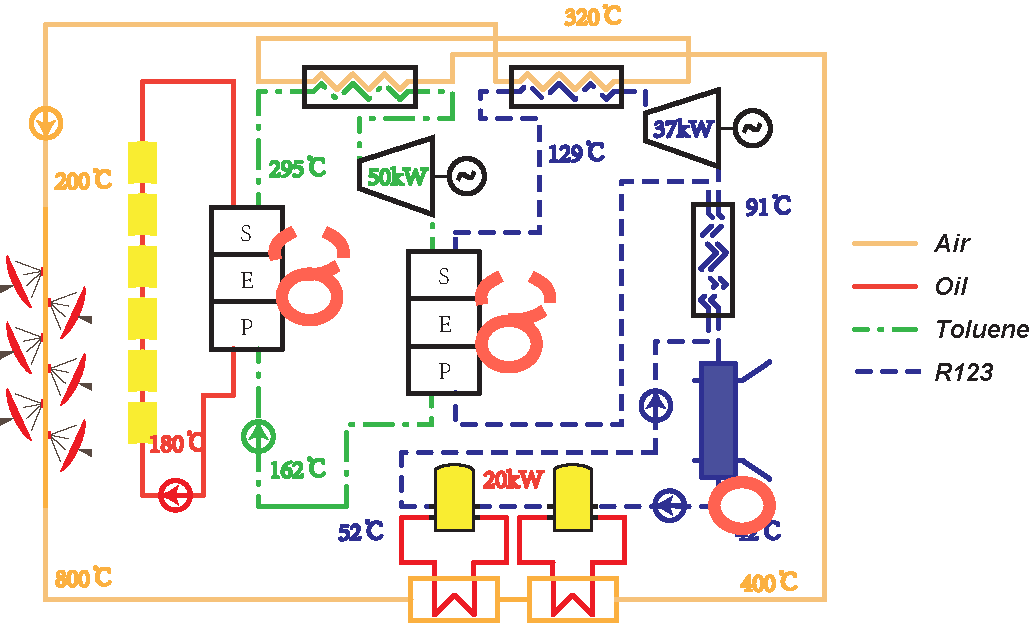
\includegraphics[width=0.7\textwidth]{fig/Ex_CascadeSystem2}
\caption{采用多级朗肯循环的一个计算案例}
\label{fig:Ex_CascadeSystem2}
\end{figure}

本文将重点分析这两个梯级系统。但是,考虑到水工质朗肯循环的应用更加广泛,其更有利于实现太阳能光热发电的大规模利用,下面的章节将使用\autoref{fig:CascadeSystem1}中的系统作为主要研究内容。

\newpage
\section{本章小结}
%This chapter systematically introduces a number of considerations in cascade solar thermal system design. These considerations include Rankine cycle fluid type, solar chimney, collector series connection, direct steam generation, heat exchanger between circuits and heat recovery between cycles. 
本章系统地研究了太阳能梯级集热发电的拓扑结构,考虑了朗肯循环结构的选择、与太阳能烟囱技术的集成、多种集热方式的集成、朗肯循环与斯特林循环的集成等方案。
接着,本文结合梯级系统的研究内容,并考虑到梯级示范系统的建设工作,针对各方案进行了详细分析,提出了两种适用于太阳能梯级集热发电的典型的系统拓扑结构。这两种典型的系统拓扑具有以下特点:

\begin{itemize}
%  \item Multiple types of collectors are applied.
  \item 使用了多种型式的集热器。
%  \item Multiple kinds of thermodynamic cycles are applied. 
  \item 使用了多个热力循环。
%  \item Air-water heat exchanger is applied to increase the Rankine cycle efficiency.
  \item 使用了空气-水换热器来提高朗肯循环的效率。
%  \item Condensate for Stirling engine cooling to recover the heat rejected by the engine.
  \item 使用朗肯循环的凝结液来冷却斯特林机。
\end{itemize}

值得注意的是,系统拓扑设计的一些考虑方案有待后续工作进一步研究。例如,塔式太阳能发电技术与槽式集热器和平板式集热器的集成方案,该方案的系统结构如\autoref{fig:seriesCollection}所示。该拓扑结构有效地利用了各种集热器的工作特性,有利于提升系统的效率并降低系统成本。